\section{Ergebnisse}

\begin{frame}[plain]
    % \frametitle{Ergebnisse}
    \centering
    \Large
    \textbf{Ergebnisse}
    \vspace{1cm}
    \begin{itemize}
        \item numerische Lösung der Selbstkonsistenzgleichung
        \begin{itemize}
            \item[$\rightarrow$] Kombination aus Newton-Verfahren (Nullstellenverfahren) und Fixpunktiteration
        \end{itemize}
        % \item 
    \end{itemize}
\end{frame}

\begin{frame}
    \frametitle{Temperaturabhängigkeit}
    \begin{minipage}[t]{0.5\textwidth}
        \begin{itemize}
            \item $W$ = $6t = $ Bandbreite, $E_D = \hbar \omega_D$ 
            \item starke Abhängigkeit von $\mu$ 
            \item Plateau für $\Delta(T)$ bei $T \rightarrow 0$
            \item Wurzelverhalten für $\Delta(T)$ bei $T \rightarrow T_C$
            \begin{itemize}
                \item[$\rightarrow$] typisch für BCS-Theorie 
            \end{itemize}
        \end{itemize}
    \end{minipage}
    \begin{minipage}[t]{0.49\textwidth}
        \begin{figure}[htbp]
            \centering
            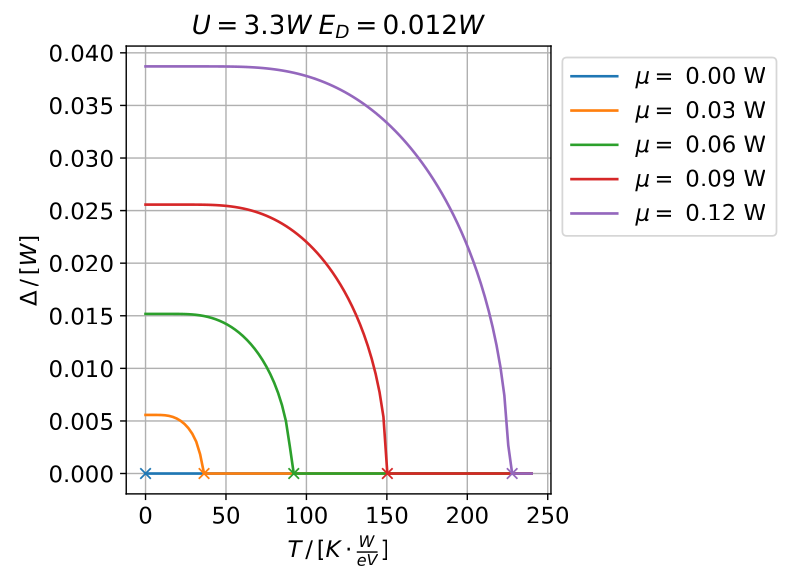
\includegraphics[width=\textwidth]{images/T_abh.png}
            % \caption{}
            % \label{<label>}
        \end{figure}
    \end{minipage}
\end{frame}

\begin{frame}
    \frametitle{Abhängigkeit von Wechselwirkung $U$}
    \begin{minipage}[t]{0.5\textwidth}
        \begin{itemize}
            \item $T=0$ ($\Delta_0$)
            \item Für $\mu \neq 0$ ist exponentieller Abfall für $U \rightarrow 0$ zu beobachten
            \item Für $\mu = 0$ (halbe Füllung) ist erst ab $U > U_C = 12,3 W$ eine Energielücke $\Delta_0 \neq 0$ vorhanden
            \begin{itemize}
                \item[$\rightarrow$] kritische Wechselwirkung existiert (``quantenkritischer Punkt'')
            \end{itemize}
        \end{itemize}
    \end{minipage}
    \begin{minipage}[t]{0.49\textwidth}
        \begin{figure}[htbp]
            \centering
            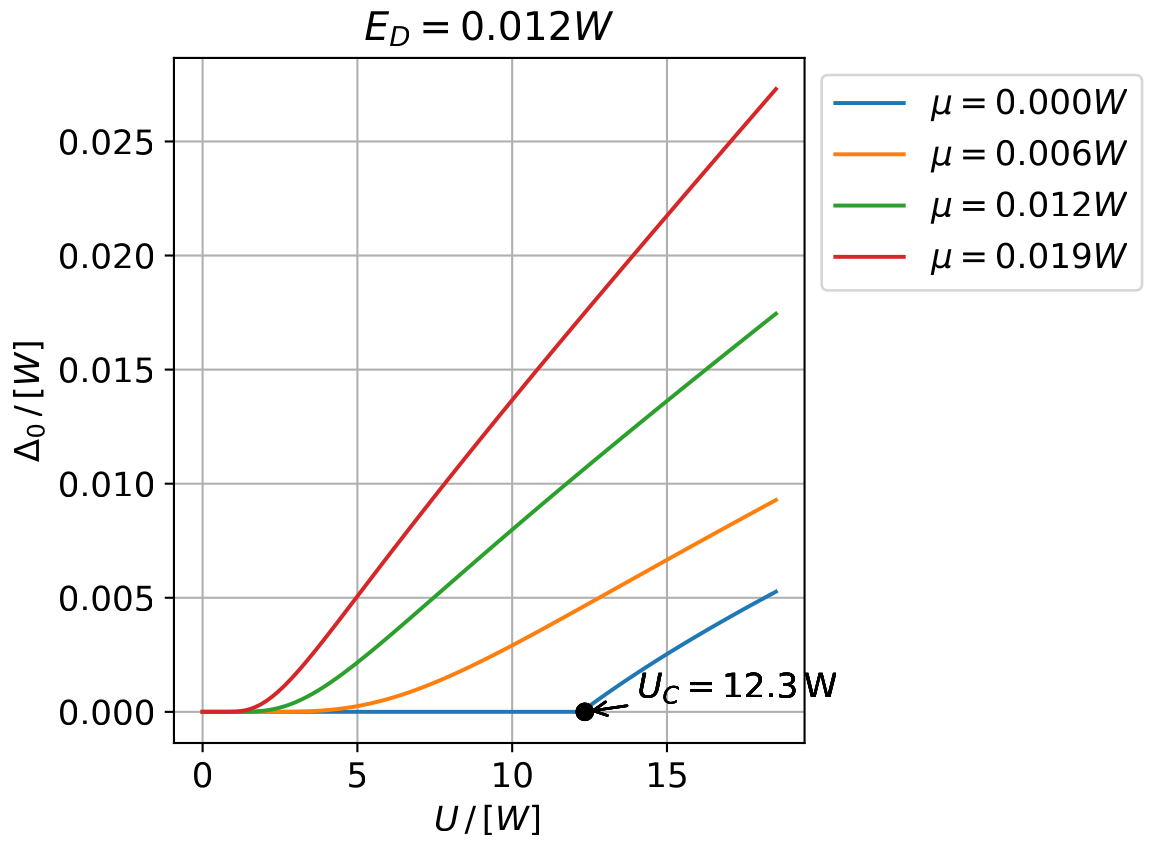
\includegraphics[width=\textwidth]{images/U_abh.png}
            % \caption{<caption>}
            % \label{<label>}
        \end{figure}
    \end{minipage}

\end{frame}

\begin{frame}
    \frametitle{Quantenkritischer Punkt}
    \begin{minipage}[t]{0.55\textwidth}
        \begin{itemize}
            \item Löse Selbstkonsistenzgleichung für $\mu = 0$ bei $T = 0$
            \begin{align*}
                1 = \frac{U}{2} \int_{-E_D}^{E_D} \frac{\rho(\epsilon)}{\sqrt{\epsilon^2 + \Delta_0^2}} \, d\epsilon
            \end{align*}
            \begin{itemize}
                \item[$\rightarrow$] erhalte Ausdruck für $U(\Delta_0)$ 
                \item[$\rightarrow$] $U_C = \lim_{\Delta_0 \rightarrow 0} U(\Delta_0)$
            \end{itemize}
            \item Für $E_D \ll W$ ist Näherung $\rho(\epsilon) \approx A \abs{\epsilon}$ gut 
            \item Es folgt
            \begin{align*}
                U_C = \frac{1}{A E_D}
            \end{align*}
            \begin{itemize}
                \item[$\rightarrow$] $A = \qty{6.6447}{W^{-2}}$
            \end{itemize}
        \end{itemize}
    \end{minipage}
    \begin{minipage}[t]{0.44\textwidth}
        \begin{figure}[htbp]
            \centering
            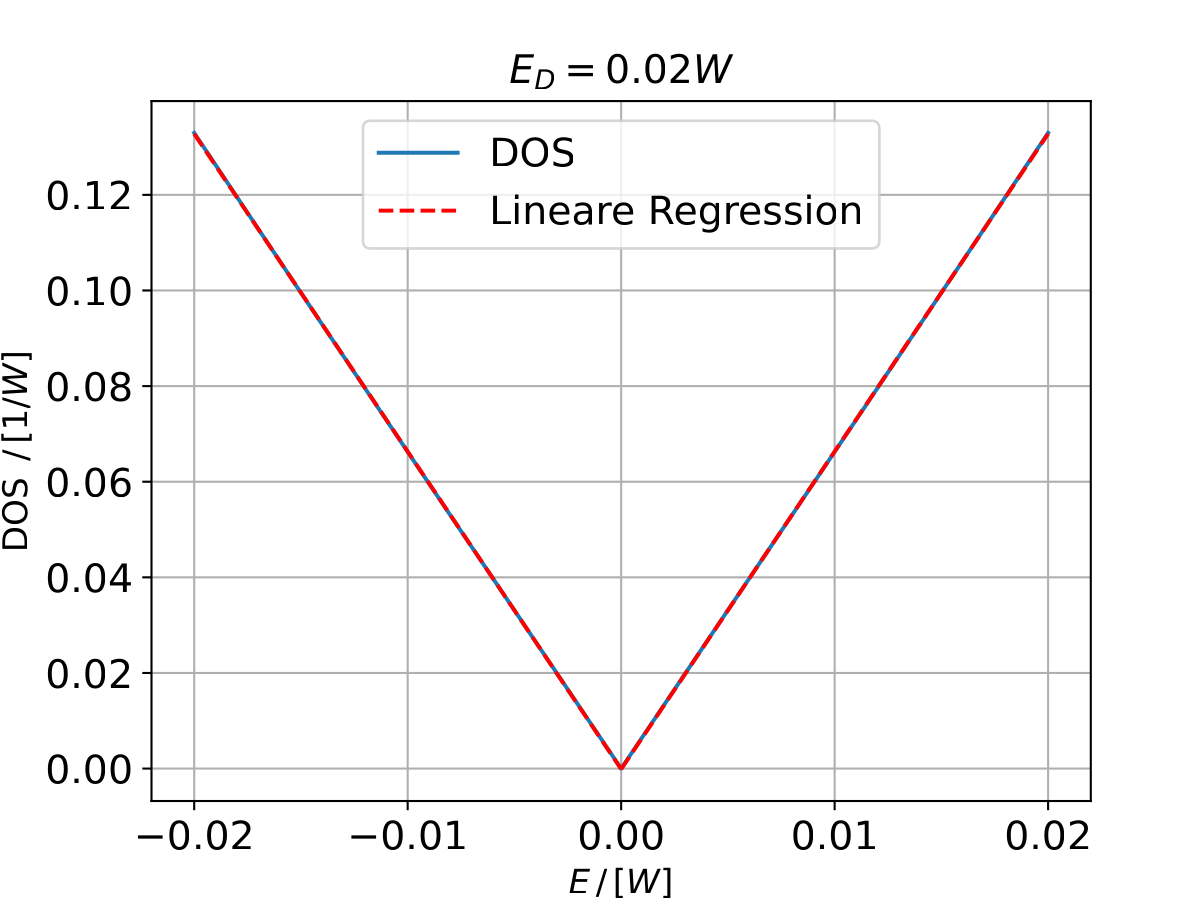
\includegraphics[width=\textwidth]{images/DOS_Regress.png}
            % \caption{<caption>}
            % \label{<label>}
        \end{figure}
    \end{minipage}
\end{frame}

\begin{frame}
    \frametitle{Abhängigkeit von Debye-Energie $E_D$}
    \begin{itemize}
            \item Hyperbolischer Verlauf von $U_C(E_D)$ bestätigt
            \item für $\mu \neq 0$ exponentieller Verlauf hier nicht erkennbar
    \end{itemize}
    \begin{minipage}[t]{0.5\textwidth}
        % \begin{itemize}
        %     \item dlad
        % \end{itemize}
        \begin{figure}[htbp]
            \centering
            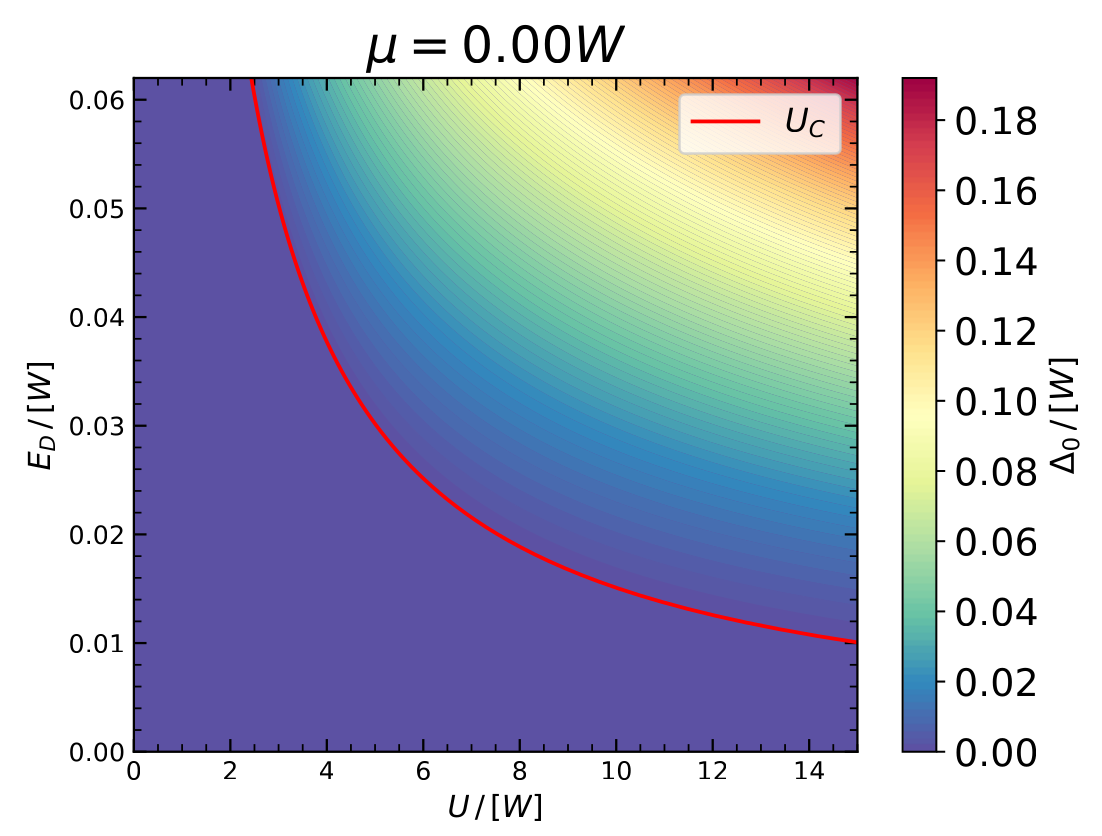
\includegraphics[width=\textwidth]{images/E_D_m0.png}
            % \caption{<caption>}
            % \label{<label>}
        \end{figure}
    \end{minipage}
    \begin{minipage}[t]{0.49\textwidth}
        \begin{figure}[htbp]
            \centering
            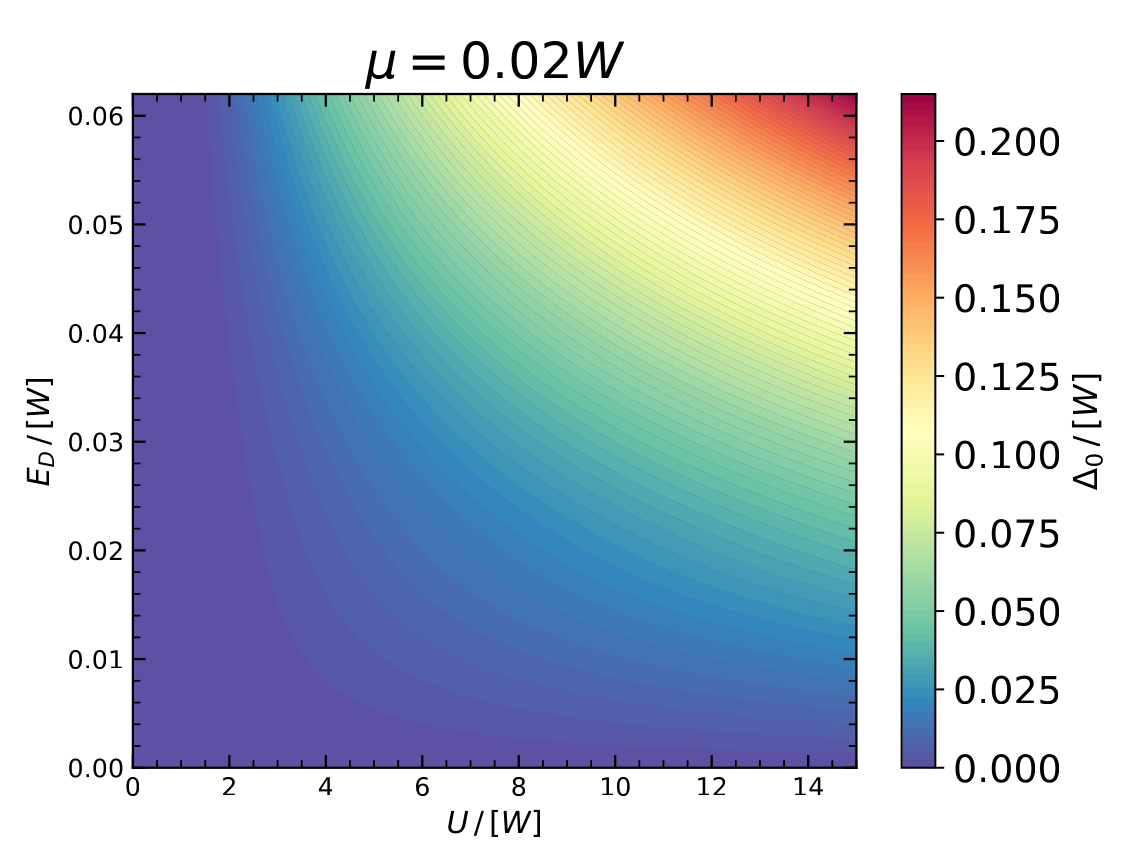
\includegraphics[width=\textwidth]{images/E_D_m1.png}
            % \caption{<caption>}
            % \label{<label>}
        \end{figure}
    \end{minipage}
\end{frame}

\begin{frame}
    \frametitle{Abhängigkeit von chemischem Potential $\mu$}
    \begin{minipage}[t]{0.5\textwidth}
        \begin{itemize}
            \item Supraleitung ist bei halber Füllung am stärksten unterdrückt
            \item Chemisches Potential bei den Van-Hove-Singularitäten ($\mu = \pm W/6$) liefert besonders starke Unterstützung 
        \end{itemize}
    \end{minipage}
    \begin{minipage}[t]{0.49\textwidth}
        \begin{figure}[htbp]
            \centering
            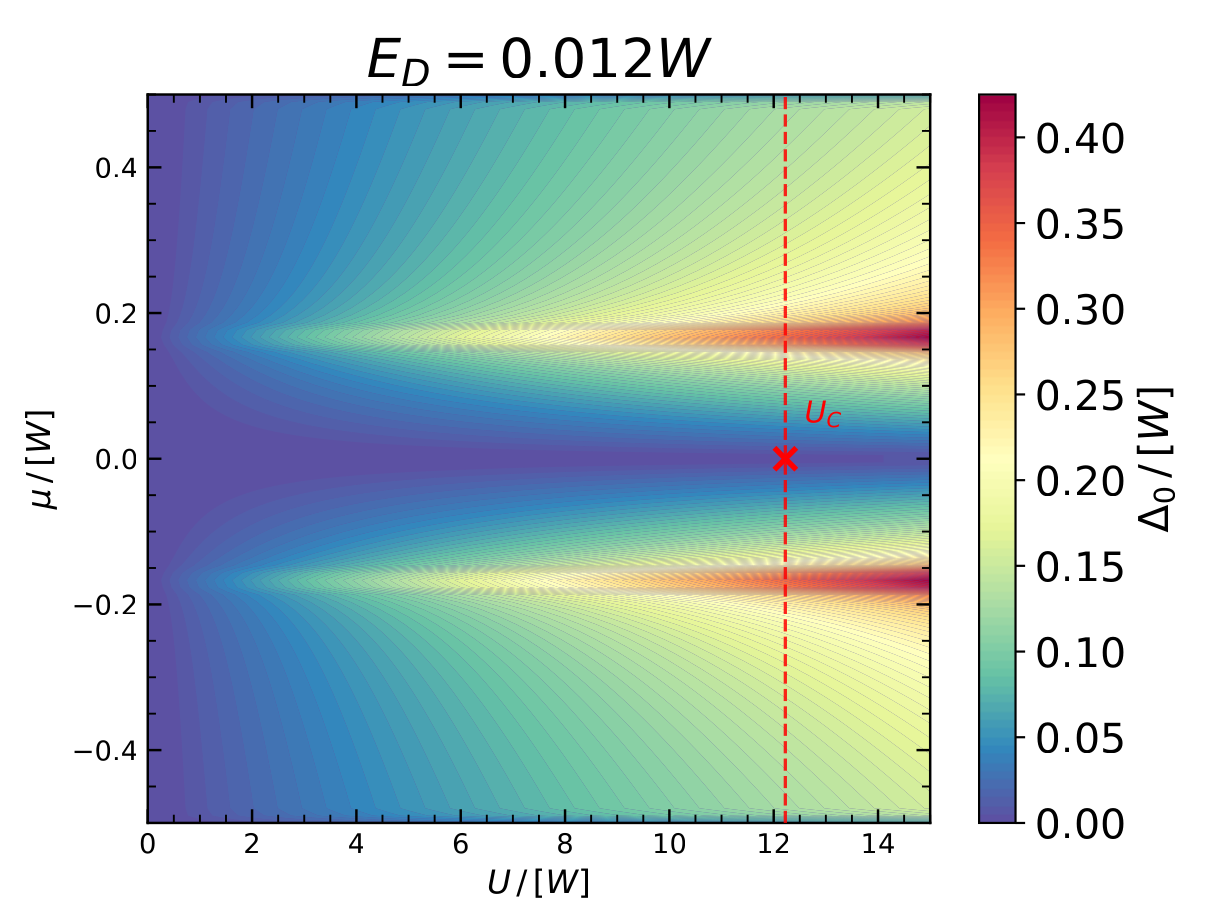
\includegraphics[width=\textwidth]{images/mu_U.png}
            % \caption{<caption>}
            % \label{<label>}
        \end{figure}
    \end{minipage}
\end{frame}


%  Zeige einmal Bandstruktur von Graphen -> Das sind die $\pi$-Bänder (relevant weil an Fermi-Energie)
% Zeige einmal wie gut NN-TB-Näherung ist (im Vergleich zu 2nd, 3rd-Neighbour)
\begin{frame}
    \frametitle{Anwendung auf Graphen -- Überblick}
    \begin{minipage}[t]{0.5\textwidth}
        \begin{itemize}
            \item Modell beschreibt $\pi$-Bänder von Graphen 
            \item Korrekturen durch höhere Tight-Binding-Terme liefern keine große Abweichung um Dirac-Punkt herum, aber Elektron-Loch-Asymmetrie
            \item bei reinem Graphen ist $\mu = 0$
            \begin{itemize}
                \item[$\rightarrow$] Veränderung von $\mu$ durch Dotierung
                % \item[$\rightarrow$] Vorhersage innerhalb dieses Modells nur ohne Annahme der Veränderung der Bandstruktur durch Dotierung möglich
            \end{itemize}
        \end{itemize}
    \end{minipage}
    \begin{minipage}[t]{0.49\textwidth}
        \begin{figure}[htbp]
            \centering
            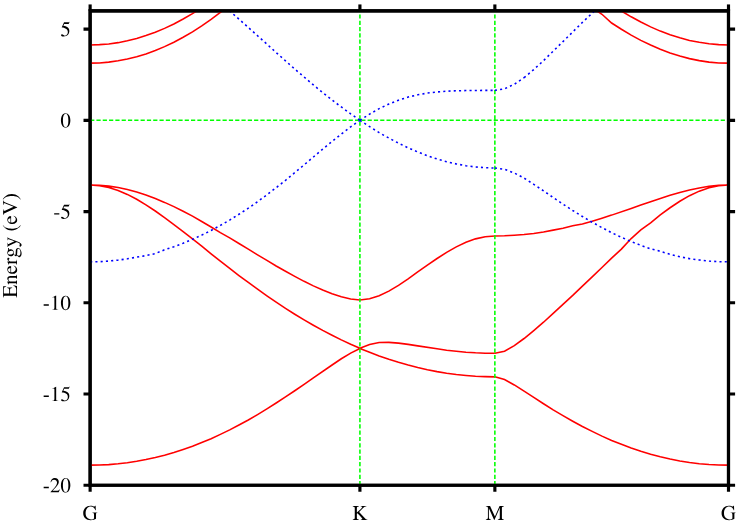
\includegraphics[width=\linewidth,height=0.44\textheight,keepaspectratio]{images/Bandstruktur_Graphen.png}
            % \caption{\scriptsize Bandstruktur Graphen~\cite{boukhvalov_hydrogen_2008}.}
        \end{figure}
        \vspace{-0.3cm}
        \begin{figure}[htbp]
            \centering
            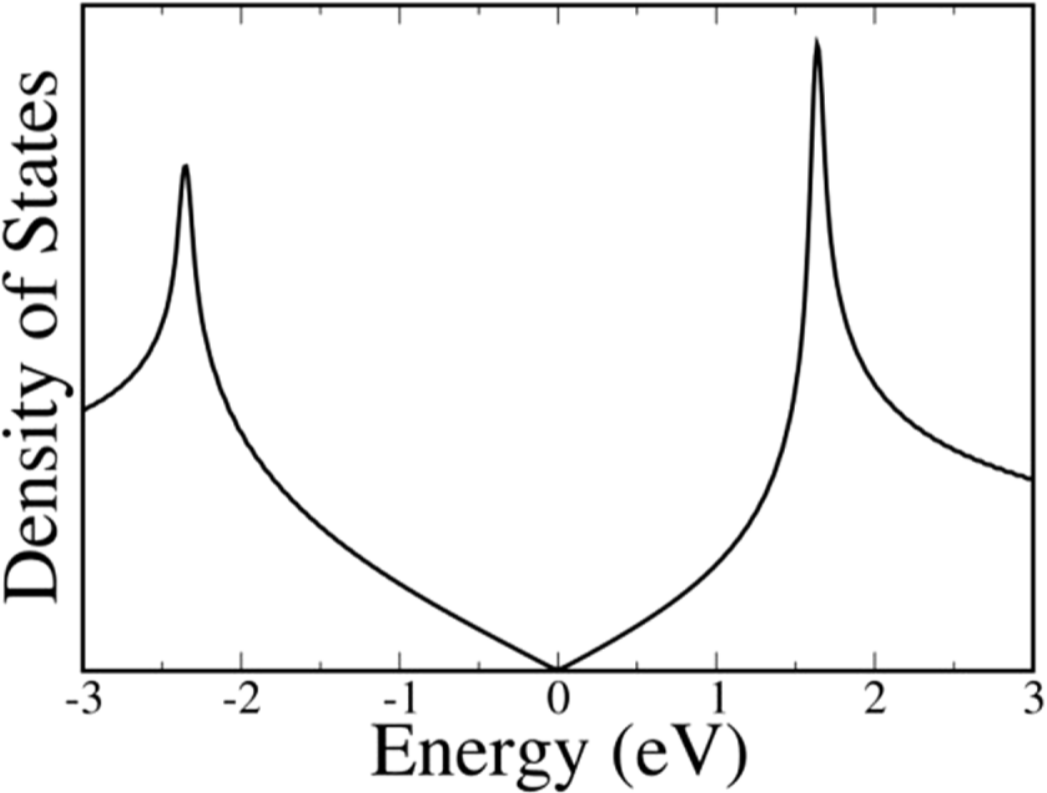
\includegraphics[width=\linewidth,height=0.44\textheight,keepaspectratio]{images/DOS_Graphen2.png}
        \end{figure}
        % \caption{Vergleich Zustandsdichte Graphen für Nächste-Nachbar und Übernächste-Nachbar Tight-Binding-Modell~\cite{castro_neto_electronic_2009}.}
    \end{minipage}
\end{frame}

\begin{frame}
    \frametitle{Anwendung auf Graphen -- Abschätzung von $U$}
    \begin{itemize}
        \item Vorhersagen von $U$ im Allgemeinen kompliziert
        \begin{itemize}
            \item[$\rightarrow$] $U$ ist Summe aus phononenvermittelter Anziehung und Coulomb-Abstoßung 
        \end{itemize}
        \item Oft wird daher $U$ anhand von gemessenen ($\Delta, T, \mu$)-Werten bestimmt
        \begin{itemize}
            \item[$\rightarrow$] nur wenig experimentelle Daten vorhanden, Supraleitung in reinem Graphen z.B. noch nicht gemessen
        \end{itemize}
        \item Größenordnung in konventionellen Supraleitern abschätzbar mit 
        \begin{align*}
            U =  -\frac{1}{\rho(0)\ln\left(\frac{\Delta_0}{2E_D}\right)}
        \end{align*}
        \begin{itemize}
            \item[$\rightarrow$] Bspw. Niob: $U \approx \qty{0.14}{eV}$
            \item[$\rightarrow$] Annahme: $U$ von Graphen weicht nicht um mehrere Größenordnungen ab
        \end{itemize}
    \end{itemize}
\end{frame}

\begin{frame}
    \frametitle{Anwendung auf Graphen -- Ergebnisse (1)}
    \begin{minipage}[t]{0.5\textwidth}
        \begin{itemize}
            \item Parameter $t = \qty{2.7}{\electronvolt}$ und $E_D = \qty{200}{\milli \electronvolt}$
            \item $U_C \approx \qty{198}{eV}$
            \begin{itemize}
                \item[$\rightarrow$] keine Supraleitung in reinem Graphen
            \end{itemize}
        \end{itemize}
    \end{minipage}
    \begin{minipage}[t]{0.49\textwidth}
        \begin{figure}[htbp]
            \centering
            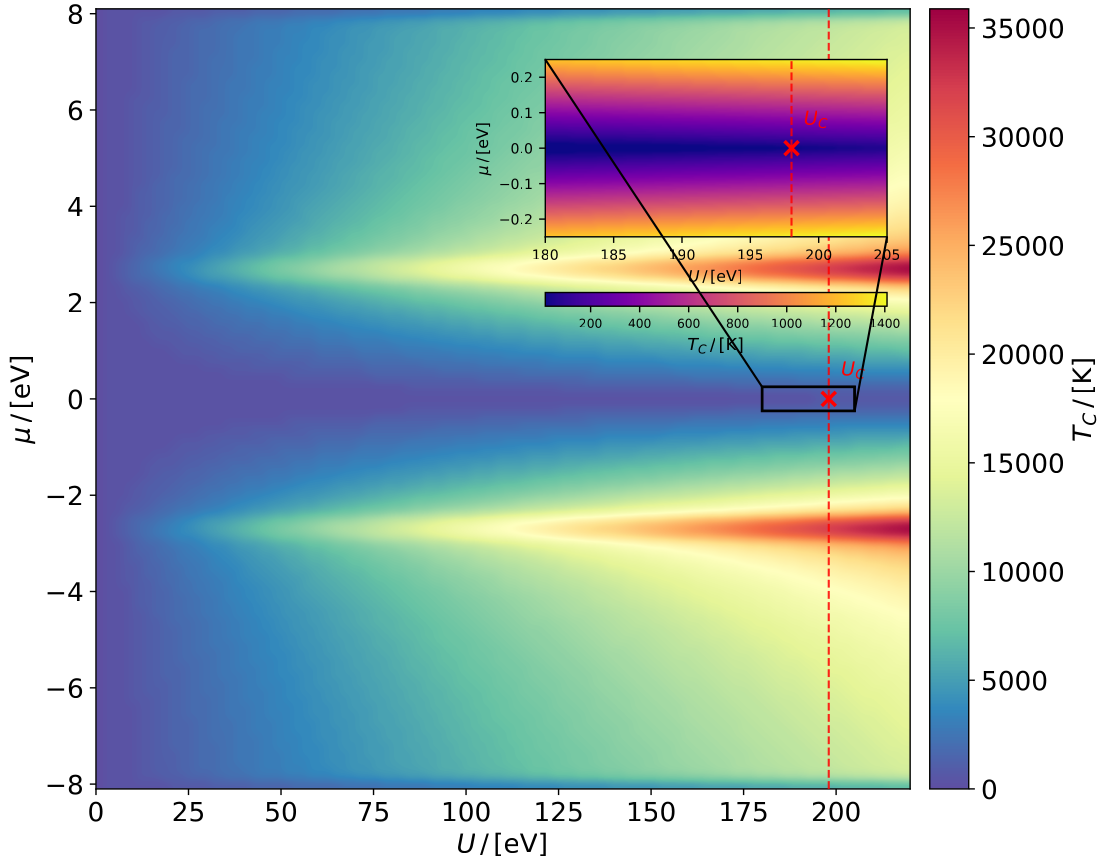
\includegraphics[width=\textwidth]{images/U_mu_Graphen2.png}
            % \caption{<caption>}
            % \label{<label>}
        \end{figure}
    \end{minipage}
\end{frame}

% \begin{frame}
%     \frametitle{Anwendung auf Graphen -- Ergebnisse (2)}
%     \begin{minipage}[t]{0.5\textwidth}
%         \begin{itemize}
%             \item Parameter $t = \qty{2.7}{\electronvolt}$ und $E_D = \qty{200}{\milli \electronvolt}$
%             \item Bei Dotierung zur Van-Hove-Singularität ist Supraleitung 
%         \end{itemize}
%     \end{minipage}
%     \begin{minipage}[t]{0.49\textwidth}
%         \begin{figure}[htbp]
%             \centering
%             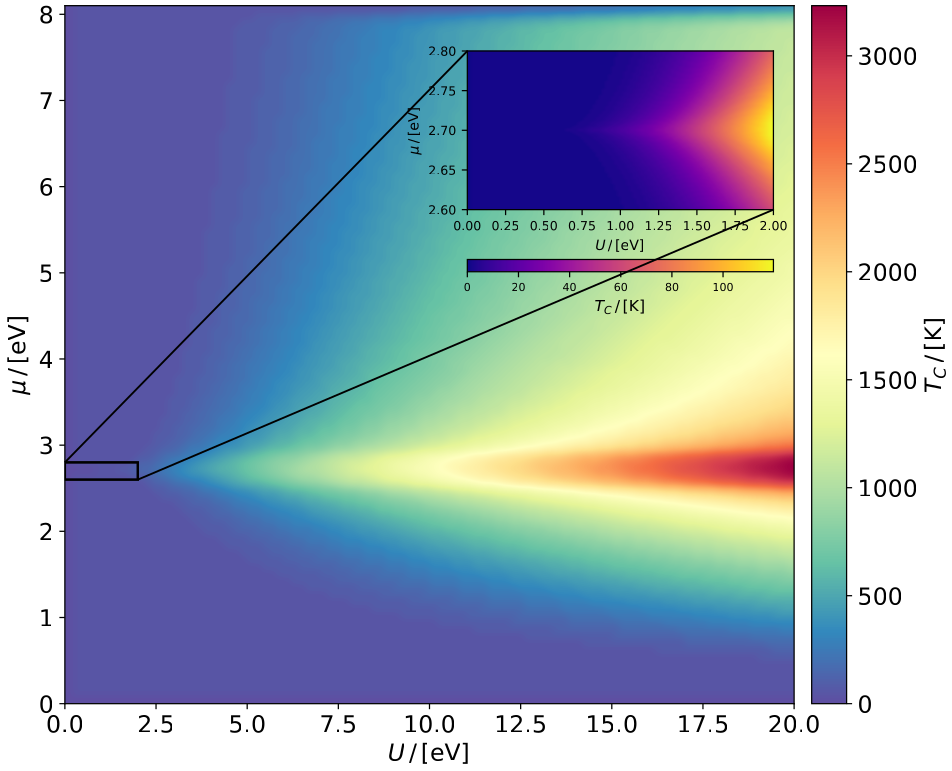
\includegraphics[width=\textwidth]{images/U_mu_Graphen.png}
%             % \caption{<caption>}
%             % \label{<label>}
%         \end{figure}
%     \end{minipage}
% \end{frame}

\begin{frame}
    \frametitle{Anwendung auf Graphen -- Ergebnisse (2)}
    \begin{minipage}[t]{0.5\textwidth}
        \begin{itemize}
            \item Untersuchung der Van-Hove-Singularität (VHS)
            \item Für $U < \qty{1}{eV}$ werden kritische Temperaturen von $T_C \geq \qty{1}{\kelvin}$ erreicht
            \begin{itemize}
                \item[$\rightarrow$] ist in der Größenordnung von $U_\text{Niob} \approx \qty{0.14}{eV}$ 
            \end{itemize} 
            \only<2>{\item Vergleich mit experimentellen/theoretischen Vorhersagen
            \begin{itemize}
                \item[$\rightarrow$] Herrera et al.~\cite{herrera_topological_2024} sagen $T_C = \qty{600}{\milli\kelvin}$ bei Dotierung bis zur VHS voraus (Modell basierend auf ARPES-Messung)
                \item[$\rightarrow$] Ludbrook et al.~\cite{ludbrook_evidence_2015} messen $\Delta = \qty{0.9}{meV}$ in Li-dotiertem Graphen (ARPES)
                \item[$\rightarrow$] beide Quellen: Bei starker Dotierung flachen Bänder ab und VHS verbreitert sich
            \end{itemize}
            \item[$\implies$] Modellvorhersagen eher qualitativ, nicht quantitativ}
        \end{itemize}
    \end{minipage}
    \begin{minipage}[t]{0.49\textwidth}
        \begin{figure}[htbp]
            \centering
            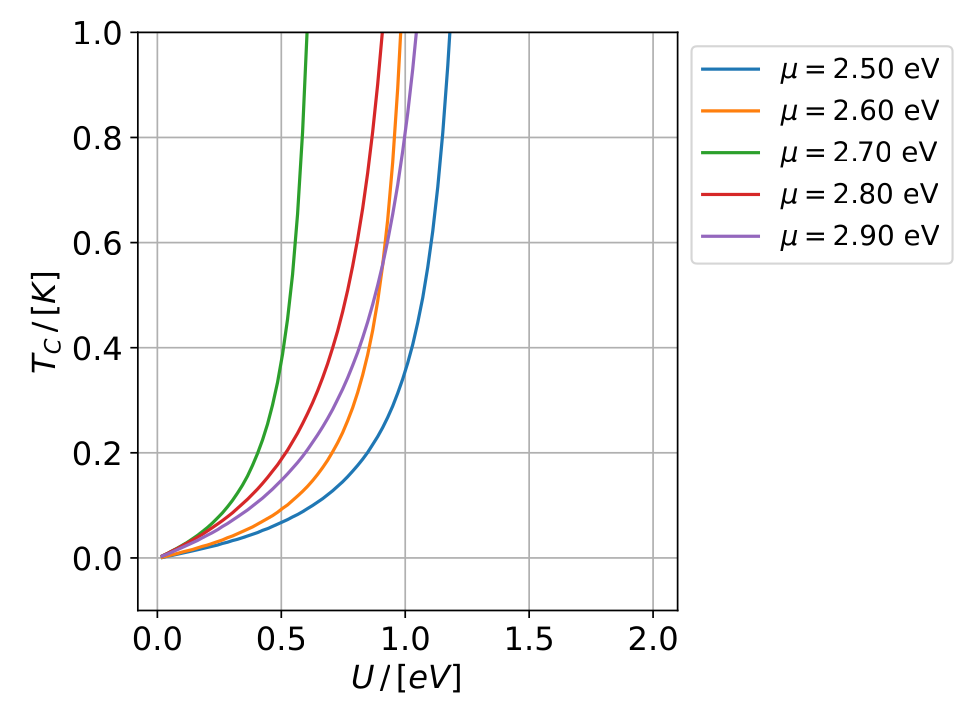
\includegraphics[width=\textwidth]{images/U_T_C.png}
        \end{figure}
    \end{minipage}
\end{frame}